\chapter{METODOLOGÍA DE LA INVESTIGACIÓN}
\section{Diseño de la investigación}
En este segmento del documento se explica cuál fue el tipo y enfoque del trabajo de investigación, al igual que la población y la muestra.


\subsection{Tipo de Investigación}
La investigación es de tipo no experimental la base de datos ya está disponible y contiene las etiquetas necesarias para entrenar y evaluar tu modelo. Ademas, que la investigación se llevará a cabo utilizando los datos disponibles , enfocándose en descubrir y explotar las relaciones entre las características de las imágenes y la clasificación de cáncer.

Mientras que el diseño de la investigación seria transversal y correlaciones. Debido a que la recolección de datos será en un solo periodo te tiempo y se centrará en identificar y explorar las relaciones entre las características de las imágenes y la clasificación de cáncer




\subsection{Enfoque de investigación}
El presente trabajo tuvo un enfoque cuantitativo debido a que al usar herramientas de deep learning y visión por computadora se realizara el procesamiento de grandes cantidades de datos. Al mismo tiempo que se empleara técnicas estadísticas para evaluar el modelo.



\section{Población y muestra}

\begin{center}
	\begin{tabular}{|p{4cm}|p{8cm}|}
		\hline
		Población & Personas con lesiones cutáneas, específicamente aquellas que presentan diferentes tipos de cáncer de piel y otras afecciones dermatológicas.  \\
		\hline
		Muestra & El conjunto de datos contiene un total de 10,015 imágenes de dermatoscopia de lesiones cutáneas. \\
		\hline
		Unidad de análisis & Cada imagen de dermatoscopia es una unidad de análisis. Estas imágenes representan diferentes tipos de lesiones cutáneas.  \\
		\hline
	\end{tabular}
\end{center}


%\section{Operacionalizacion de variables}




\section{Técnicas de recolección}

La Base de datos que se utilizara para este trabajo es Skin Cancer MNIST: HAM10000, la que es una colección de múltiples imagenes dermatológicas del año 2018. Las variables se clasifican en tipos de lesión cutánea(melanoma/no melanoma). El tipo de análisis que se realizara es la clasificación y categorización las imágenes de acuerdo con los diferentes tipos de lesiones cutáneas.

\begin{figure}[h]
	\begin{center}
		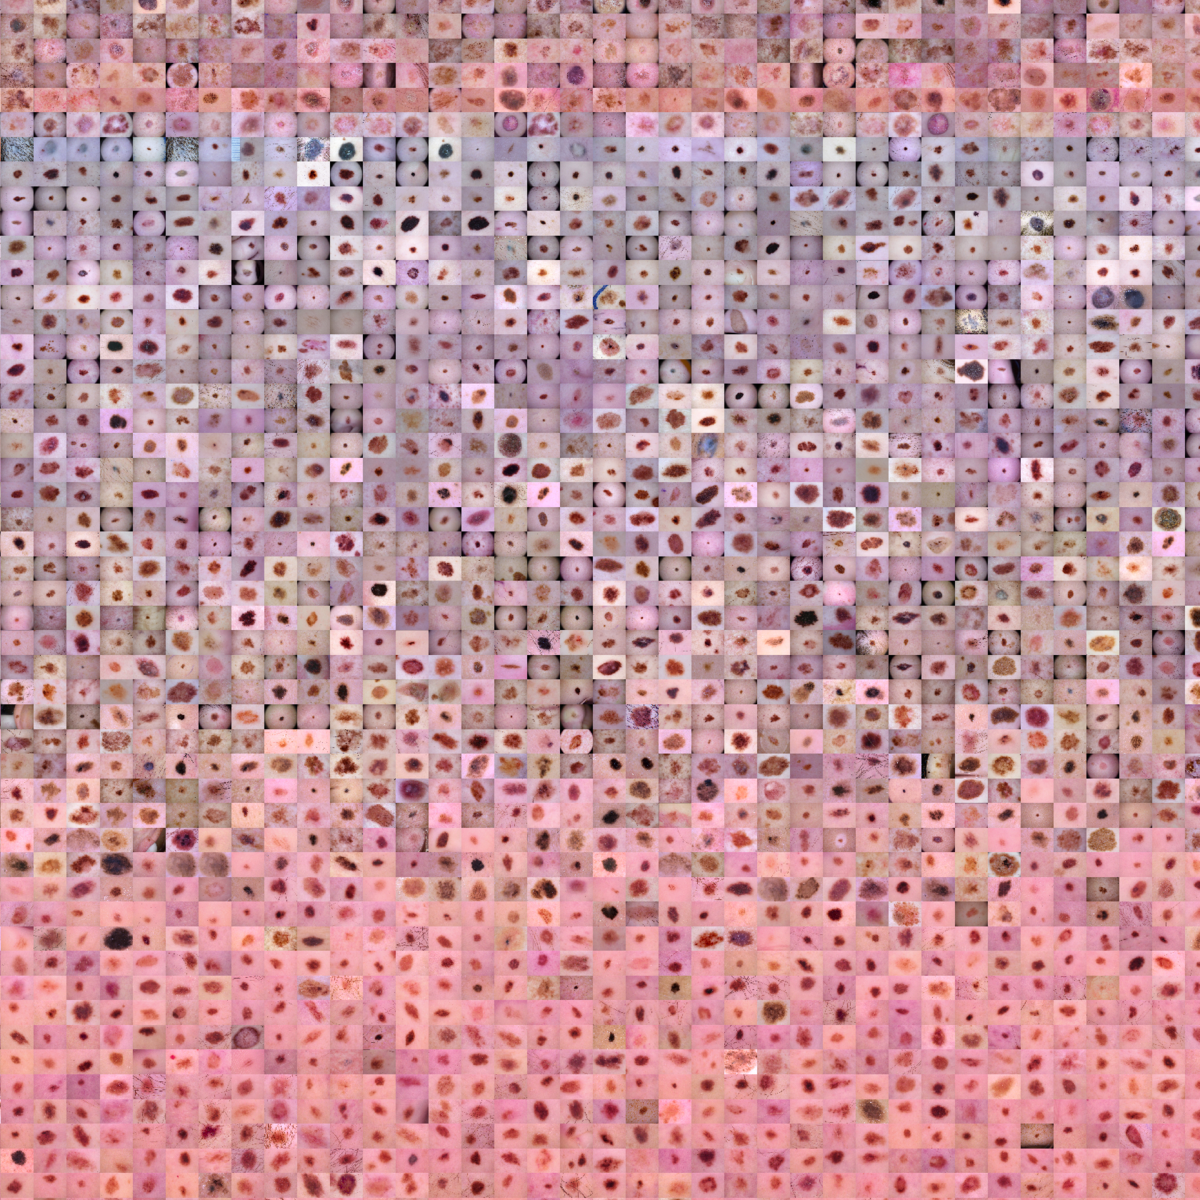
\includegraphics[width=0.25\textwidth]{3/figures/dataset-card.png}
		\caption{Imagén de la Base de Datos. Fuente: \cite{kaggleSkinCancer}}
		\label{1:fig 17}
	\end{center}
\end{figure}





\section{Técnicas para el procesamient y análisis de la información}

\subsection{Metodología de la implementación de la solución}

Para escoger la metodología, se realizó una investigación de las metodologías usadas en los antecedentes presentados con la finalidad de cuál es la que conviene usar más. No obstante, estos solo mencionan los pasas de su metodología, pero no el nombre de este. 

Aun así según la información recolectada se decido implementar la metodología Iterativa. Estas por las siguentes puntos:

- División del trabajo: Permite realizar una división según las partes del proyecto, facilitando la gestión y su seguimiento.

- ttavilidad: Se le puede realizar ajustes si el proyecto lo necesita

\begin{figure}[h]
	\begin{center}
		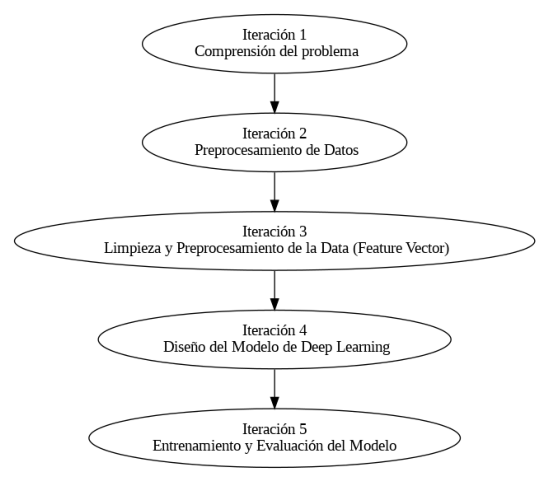
\includegraphics[width=0.5\textwidth]{3/figures/metodologia.png}
		\caption{Imagén de la Base de Datos. Fuente: Elavoracion propia}
		\label{1:fig 19}
	\end{center}
\end{figure}



	






\subsubsection{Metodología para la medición de resultados}

Para evaluar la performance de un modelo, se utilizan diversas métricas como instrumentos de medición de desempeño a partir de los resultados arrojados en la Matriz de confusión. A continuación, se detalla su concepto y sus elementos.


La fórmula de Precisión (Accuracy) se define como:
 
\begin{equation}
	\text{Precisión} = \frac{TP + TN}{TP + TN + FP + FN}
\end{equation}

Esta formula sera usada para la precisio del algoritmo.





\section{Cronograma de actividades}

Se elaboró un cronograma de actividades de toda la investigación, mostrada en la Figura \ref{3:fig13}, contemplando desde el inicio del año 2024 hasta finales del 2024 deonde se realizara la sustentacion del trabajo sustentación del trabajo.

\begin{figure}[h]
	\begin{center}
		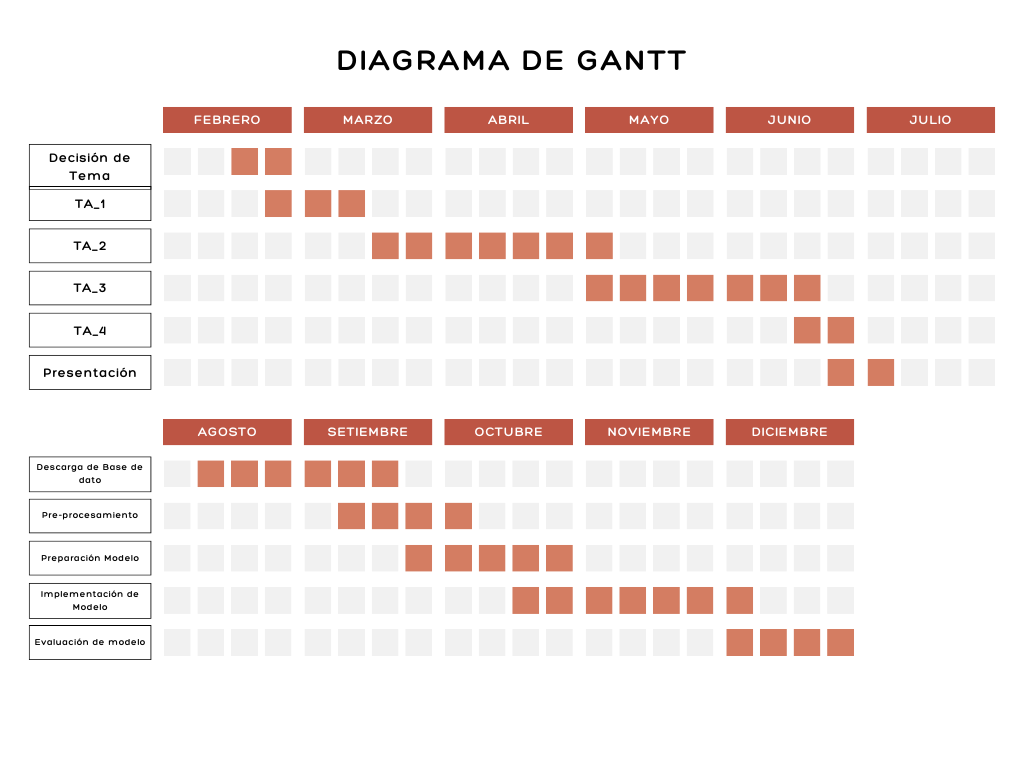
\includegraphics[width=1\textwidth]{3/figures/Cronograma Diagrama de Gantt.png}
		\caption{Diagrama de Grantt. Fuente: Elavoración Propia }
		\label{1:fig 18}
	\end{center}
\end{figure}




\section{Presupuesto}

\begin{center}
	\begin{tabular}{|p{8cm}|p{3cm}|}
		\hline
		Materiales & Costos  \\
		\hline
		Computadora Core i7 & 2000 \\
		\hline

		Total & 2000 \\
		\hline
	\end{tabular}
\end{center}


\begin{comment}
\begin{table}[h!]
	\centering
	\begin{tabular}{|l|p{10cm}|}
		\hline
		\textbf{Concepto} & \textbf{Descripción} \\ \hline
		Población & Personas con lesiones cutáneas, específicamente aquellas que presentan diferentes tipos de cáncer de piel y otras afecciones dermatológicas. \\ \hline
		Muestra & El conjunto de datos contiene un total de 10,015 imágenes de dermatoscopia de lesiones cutáneas. \\ \hline
		Unidad de análisis & Cada imagen de dermatoscopia es una unidad de análisis. Estas imágenes representan diferentes tipos de lesiones cutáneas. \\ \hline
		Variable y tipo de análisis & Clase de la lesión cutánea (melanoma/no melanoma). Clasificación y categorización de las imágenes de acuerdo a los diferentes tipos de lesiones cutáneas. \\ \hline
	\end{tabular}
	
	\label{tabla:dataset}
\end{table}
\end{comment}


\begin{comment}

 Nisi porta lorem mollis aliquam ut porttitor leo. Aenean pharetra magna ac placerat vestibulum. Est placerat in egestas erat imperdiet sed euismod. Velit euismod in pellentesque massa placerat. Enim praesent elementum facilisis leo vel fringilla. Ante in nibh mauris cursus mattis molestie a iaculis. Erat pellentesque adipiscing commodo elit at imperdiet dui accumsan sit. Porttitor lacus luctus accumsan tortor posuere ac ut. Tortor at auctor urna nunc id. A iaculis at erat pellentesque adipiscing commodo elit. La Figura \ref{fig1} y el Cuadro \ref{tab:widgets}

	\begin{figure}[h]
		\begin{center}
			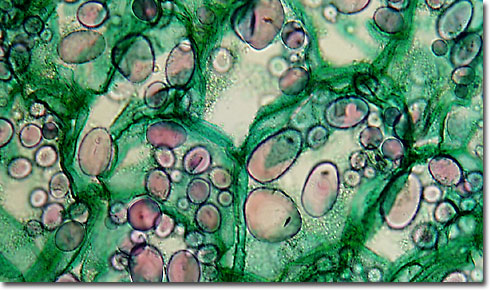
\includegraphics[width=0.8\textwidth]{3/figures/largepotato.jpg}
			\caption{Prueba de Figura}
			\label{fig1}
		\end{center}
		
	\end{figure}


\section{Operacionalización de Variables}

Nisi porta lorem mollis aliquam ut porttitor leo. Aenean pharetra magna ac placerat vestibulum. Est placerat in egestas erat imperdiet sed euismod. Velit euismod in pellentesque massa placerat. Enim praesent elementum facilisis leo vel fringilla. Ante in nibh mauris cursus mattis molestie a iaculis. Erat pellentesque adipiscing commodo elit at imperdiet dui accumsan sit. Porttitor lacus luctus accumsan tortor posuere ac ut. Tortor at auctor urna nunc id. A iaculis at erat pellentesque adipiscing commodo elit.
\section{Instrumentos de medida}
Nisi porta lorem mollis aliquam ut porttitor leo. Aenean pharetra magna ac placerat \begin{itemize}
	\item muscle and fat cells remove glucose from the blood,
	\item cells breakdown glucose via glycolysis and the citrate cycle, storing its energy in the form of ATP,
	\item liver and muscle store glucose as glycogen as a short-term energy reserve,
	\item adipose tissue stores glucose as fat for long-term energy reserve, and
	\item cells use glucose for protein synthesis.
\end{itemize}

\section{Técnicas de recolección de datos}
Nisi porta lorem mollis aliquam ut porttitor leo. Aenean pharetra magna ac placerat vestibulum. Est placerat in egestas erat imperdiet sed euismod. Velit euismod in pellentesque massa placerat. Enim praesent elementum facilisis leo vel fringilla. Ante in nibh mauris cursus mattis molestie a iaculis. Erat pellentesque adipiscing commodo elit at imperdiet dui accumsan sit. Porttitor lacus luctus accumsan tortor posuere ac ut. Tortor at auctor urna nunc id. A iaculis at erat pellentesque adipiscing commodo elit.

\LaTeX{} is great at typesetting mathematics. Let $X_1, X_2, \ldots, X_n$ be a sequence of independent and identically distributed random variables with
\begin{equation}
	S_n = \frac{X_1 + X_2 + \cdots + X_n}{n}
	= \frac{1}{n}\sum_{i}^{n} X_i
	\label{eq1}
\end{equation}

La Ecuación \ref{eq1} denote their mean. Then as $n$ approaches infinity, the random variables $$\sqrt{n}(S_n - \mu)$$ converge in distribution to a normal $\mathcal{N}(0, \sigma^2)$.

\section{Técnicas para el procesamiento y análisis de la información}
Nisi porta lorem mollis aliquam ut porttitor leo. Aenean pharetra magna ac placerat vestibulum. Est placerat in egestas erat imperdiet sed euismod. Velit euismod in pellentesque massa placerat. Enim praesent elementum facilisis leo vel fringilla. Ante in nibh mauris cursus mattis molestie a iaculis. Erat pellentesque adipiscing commodo elit at imperdiet dui accumsan sit. Porttitor lacus luctus accumsan tortor posuere ac ut. Tortor at auctor urna nunc id. A iaculis at erat pellentesque adipiscing commodo elit.

You can make lists with automatic numbering \dots

\begin{enumerate}
	\item Like this,
	\item and like this.
\end{enumerate}
\dots or bullet points \dots
\begin{itemize}
	\item Like this,
	\item and like this.
\end{itemize}


\section{Cronograma de actividades y presupuesto}
Nisi porta lorem mollis aliquam ut porttitor leo. Aenean pharetra magna ac placerat vestibulum. Est placerat in egestas erat imperdiet sed euismod. Velit euismod in pellentesque massa placerat. Enim praesent elementum facilisis leo vel fringilla. Ante in nibh mauris cursus mattis molestie a iaculis. Erat pellentesque adipiscing commodo elit at imperdiet dui accumsan sit. Porttitor lacus luctus accumsan tortor posuere ac ut. Tortor at auctor urna nunc id. A iaculis at erat pellentesque adipiscing commodo elit.

\begin{table}[h]
	\centering
	\begin{tabular}{l|r}
		Item & Quantity \\\hline
		Widgets & 42 \\
		Gadgets & 13
	\end{tabular}
	\caption{\label{tab:widgets}An example table.}
\end{table}

\end{comment}

